\section{Task 3: Real-Time Communication Flow Classification}
\label{sec:task3}

\subsection{Problem and Data}
\label{sec:t3-problem}

Given only the first five packets of a real-time communication (RTC) flow (packet
lengths and relative timestamps), the system must predict which of five applications
(Discord, Google Meet, Messenger, WhatsApp, Zoom) produced the flow and whether it is a
voice or a video call, giving ten classes. The organisers report accuracy, precision,
recall and F$_\beta$; for our submission recall equals accuracy, which points to
support-weighted averaging. During development we optimised macro-F1, which weights
the small classes (40 Google Meet voice flows) as much as the large ones (256 Discord
video flows).

There are 1{,}285 training and 327 test flows (Table~\ref{tab:t3-data} in
Appendix~\ref{app:t3}), and train and test are exchangeable (adversarial-validation
AUC 0.529; Exp.~C1). Three properties dominate the design space: no call identifier is
released although flows from the same call are near-duplicates (an estimated
$\approx$400 source calls); more than half of all flows (56.5\%) have a window in which
every packet is below 300 bytes, i.e.\ only audio-sized packets whatever the call
mode; and the dataset is small.

\subsection{Submitted System}
\label{sec:t3-arch}

\begin{figure}[t]
\centering
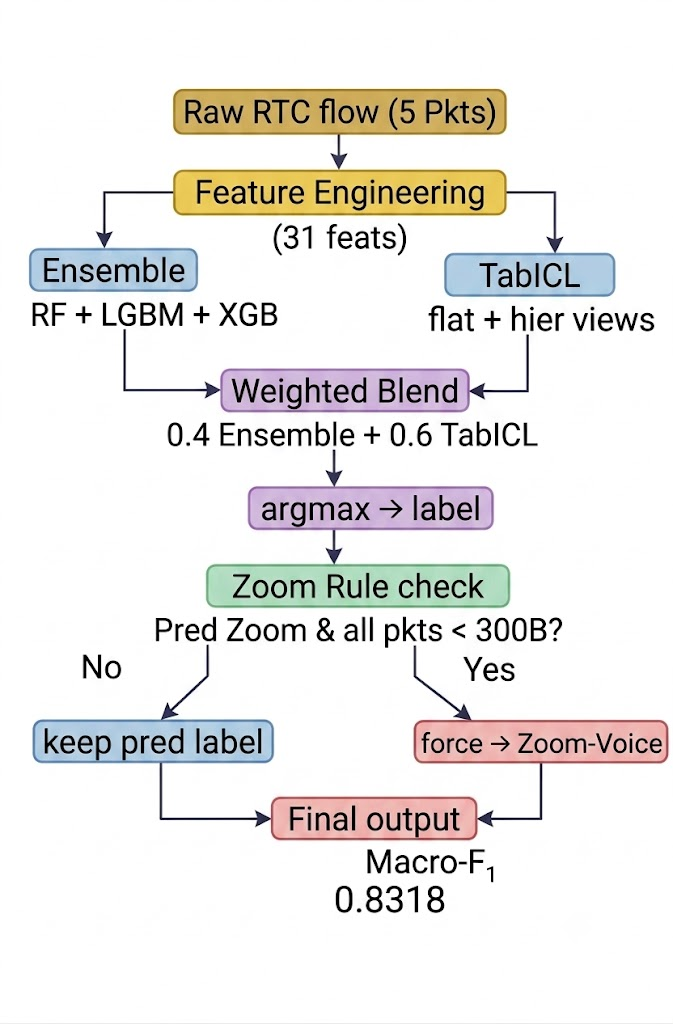
\includegraphics[width=0.36\textwidth]{task3_architecture.png}
\caption{Task~3 pipeline: 31 columns feed the tree ensemble (Branch~A) and 241
columns feed TabICL in flat and hierarchical views (Branch~B); the probabilities are
blended $0.4/0.6$, and a parameter-free rule sends audio-only Zoom windows to
Zoom\_voice.}
\label{fig:t3-arch}
\end{figure}

The pipeline (Fig.~\ref{fig:t3-arch}) has five stages and two feature
representations.


\noindent\textbf{Stage 0: features.} Branch~A uses 31 compact columns: five lengths, four
timestamps, four length differences, four inter-arrival gaps, the lengths in rank
order, argmax/argmin position, range, mean, standard deviation, median and total span,
plus the logarithm of the fourth packet length and the position of the largest
packet-to-packet size increase. Branch~B uses 241 deterministic columns (raw and log
values, inter-arrival and length statistics, sequence shape, protocol bands and
residues, burst structure, rate and spectral terms). No feature depends on labels.

\noindent\textbf{Stage 1: Branch A, tree ensemble.} RandomForest~\cite{breiman2001rf} (600 trees,
balanced-subsample weights), LightGBM~\cite{ke2017lightgbm} (400 trees, depth 4, 15
leaves, learning rate 0.05, balanced) and XGBoost~\cite{chen2016xgboost} (400 trees,
depth 4, learning rate 0.05, subsample and column sample 0.8). Probabilities are
averaged with equal weight, softened by a temperature $T=2$
($\tilde p_k\propto\bar p_k^{1/T}$), divided by the empirical class prior
$\hat\pi_k$ and renormalised. All estimators run single-threaded (Exp.~C9).

\noindent\textbf{Stage 2: Branch B, TabICL.} TabICL~\cite{qu2025tabicl} with 16 internal
estimators and no tuning, in a flat ten-class view and a hierarchical view (an
application head and per-application voice/video heads); the two probability vectors
are averaged.
% TODO: confirm the hierarchical view is the product P(app)*P(mode|app)

\noindent\textbf{Stage 3: blend.} $p=0.4\,p_{\mathrm{A}}+0.6\,p_{\mathrm{B}}$, then argmax. The
weight is the median of ten weights, each chosen on the training side of one grouped
fold (Exp.~C23).

\noindent\textbf{Stage 4: Zoom rule.} If the blended label is either Zoom class and all five
packet lengths are below 300 bytes, the label is set to Zoom\_voice. The rule has no
fitted parameter (Exps.~C18--C19).

\noindent\textbf{Validation protocol.} Every Branch~B selection decision is scored on
grouped folds (\texttt{StratifiedGroupKFold}, 5 splits $\times$ 2 repeats) over a
pseudo-call key, the packet-length tuple rounded to 8 bytes joined with the rounded
log-duration, which yields 1{,}107 pseudo-groups. Negative controls pass (shuffled
labels 0.1549, prior-only 0.1992; Exp.~C2). Only nested values of fitted quantities (blend
weight, offsets, biases) are used for choosing. Branch~A, developed earlier under
stratified folds, is the one exception. Unlabelled test flows are never used to fit a
label-dependent quantity.

\noindent\textbf{Submission} (Exp.~C25). Branch~A was refit on all 1{,}285 rows
\emph{without} the per-class offsets and specialist of Exp.~C7, so that the blend
receives corrected probabilities rather than outputs shifted toward recall; Branch~B
test probabilities come from a full-data refit. The rule routed 43 of the 327 test
flows to Zoom\_voice, in line with the training proportion.

\subsection{Development Path}
\label{sec:t3-experiments}

\noindent\textbf{Model search.} 2{,}377 grid points over eleven model families, followed
by Optuna~\cite{optuna}, put boosted trees ahead; distance, kernel, linear and neural
models trailed by 9--11 points (Exp.~C3). TabICL with no tuning beat the best searched
point (LightGBM, 0.8249) at every feature width, though the paired difference is not
significant (66 rows won against 49, $p=0.135$; Exp.~C10). Feature pruning,
label-aware features, pretraining on a public corpus~\cite{mirage}, probe features, a
tuple lookup and call-level aggregation did not help (Exps.~C4, C12, C13, C15).

\noindent\textbf{One pair bounds the score.} The standing tree configuration made 237
errors, 175 of them in audio-only windows and 68 between Zoom\_voice and Zoom\_video
alone (Exp.~C17). Inside audio-only windows the Zoom pair is not separable: the subset
is exactly balanced (80 voice, 80 video) and the grouped AUC of video against voice is
0.551, against 0.83--0.88 for the other applications (Exp.~C18). Even with every other
flow correct, accuracy is capped at 0.9377 and macro-F1 at 0.9364.

\noindent\textbf{A derived rule, not a fitted one.} On an evenly split, inseparable
subset every assignment has the same accuracy but not the same macro-F1: sending all
160 flows to Zoom\_voice gives F1 0.667 (voice) and 0.697 (video), against 0 and 0.811
for Zoom\_video (Exp.~C19). The rule improved macro-F1 for all six model families in
every view (Exp.~C20), whereas fitted per-class biases gained in sample and lost nested
(Exps.~C14, C21). It is neutral for accuracy (0.8233 $\rightarrow$ 0.8241).

\noindent\textbf{Two branches.} Branch~A's complementary strength is Zoom\_voice
recall (0.712 against 0.438 for Branch~B; Exp.~C22). Nested selection picked blend weights from 0.25 to 0.55 across
folds, median 0.40 (Exp.~C23). The blend improves on Branch~B with the rule by
$+0.0039$ to $+0.0072$ macro-F1, but the bootstrap interval includes zero (Exp.~C24).

\subsection{Results}
\label{sec:t3-results}

The organisers scored the submission at accuracy 0.8746, precision 0.9211, recall
0.8746 and F$_\beta$ 0.883 on the 327 test flows. Because the official metrics are
support-weighted, F$_\beta$ is not comparable with our macro-F1 estimates in
Table~\ref{tab:t3-summary}. The test accuracy is 3.6 points above the cross-validated
accuracy of the blend (0.8389); with $n=327$ the standard error of an accuracy near
0.87 is about 1.9 points, so the difference is about two standard errors. Possible
contributors are training on all 1{,}285 flows rather than four fifths and the
weighted metric favouring large classes; we did not test either.

\begin{table}[t]
\caption{Task~3 results. Cross-validation rows are pooled grouped out-of-fold
predictions (each of the 1{,}285 rows scored twice); the first two rows are single-model
references (Exps.~C3, C10).}
\label{tab:t3-summary}
\centering
\small
\begin{tabular}{lccc}
\toprule
Configuration & Accuracy & Macro-F1 & Fold mean \\
\midrule
Official test (weighted metrics, $n=327$) & \textbf{0.8746} & --- & --- \\
\midrule
Best searched point, LightGBM (C3) & 0.8249 & 0.8069 & --- \\
TabICL, default, 241 columns (C10) & 0.8389 & 0.8232 & --- \\
Branch A, corrected probabilities (stratified folds) & 0.7961 & 0.7900 & --- \\
Branch B, flat+hier average & 0.8358 & 0.8201 & 0.8175 \\
Branch B + Zoom rule & 0.8342 & 0.8292 & 0.8268 \\
Blend, nested weight, no rule & 0.8389 & 0.8319 & 0.8286 \\
Blend, nested weight, + Zoom rule (submitted) & --- & 0.8345 & \textbf{0.8318} \\
Blend, $w=0.40$, + Zoom rule$^{a}$ & 0.8389 & 0.8366 & --- \\
\midrule
\multicolumn{4}{l}{\footnotesize $^{a}$ $w$ located on the same rows (Exp.~C23); optimistic.}\\
\bottomrule
\end{tabular}
\end{table}

\noindent\textbf{Limitations.} Branch~A's out-of-fold probabilities come from
stratified rather than grouped folds, so the 0.40 weight on Branch~A is, if anything,
too high and the nested estimate of 0.8318 is likely somewhat optimistic. The Branch~B
variant, the 16-estimator setting and the blend were chosen among near-equal
candidates on the same 1{,}285 rows. The Zoom rule is a property of this dataset's Zoom
audio-only windows and is not claimed to transfer (Appendix~\ref{sec:t3-limits}).
